\documentclass[compress,red]{beamer}
\mode<presentation>
\setbeamertemplate{navigation symbols}{}

\usetheme{Warsaw}


%\hypersetup{pdfpagemode=FullScreen} % makes your presentation go automatically to full screen

% define your own colors:
\definecolor{Red}{rgb}{1,0,0}
\definecolor{Blue}{rgb}{0,0,1}
\definecolor{Green}{rgb}{0,1,0}
\definecolor{magenta}{rgb}{1,0,.6}
\definecolor{lightblue}{rgb}{0,.5,1}
\definecolor{lightpurple}{rgb}{.6,.4,1}
\definecolor{gold}{rgb}{.6,.5,0}
\definecolor{orange}{rgb}{1,0.4,0}
\definecolor{hotpink}{rgb}{1,0,0.5}
\definecolor{newcolor2}{rgb}{.5,.3,.5}
\definecolor{newcolor}{rgb}{0,.3,1}
\definecolor{newcolor3}{rgb}{1,0,.35}
\definecolor{darkgreen1}{rgb}{0, .35, 0}
\definecolor{darkgreen}{rgb}{0, .6, 0}
\definecolor{darkred}{rgb}{.75,0,0}

\xdefinecolor{olive}{cmyk}{0.64,0,0.95,0.4}
\xdefinecolor{purpleish}{cmyk}{0.75,0.75,0,0}


\useoutertheme[subsection=false]{smoothbars}


% include packages
\usepackage{subfigure}
\usepackage{multicol}
\usepackage{amsmath}
\usepackage{epsfig}
\usepackage{graphicx}
\usepackage[all,knot]{xy}
\xyoption{arc}
\usepackage{url}
\usepackage{multimedia}
\usepackage{hyperref}
\usepackage{helvet}
\usepackage[polish,english]{babel}
\usepackage[utf8]{inputenc}
\usepackage{multirow}
%%%%%%%%%%%%5
%\usepackage{geometry}
%\geometry{verbose,letterpaper}
%\usepackage{movie15}
%\usepackage{hyperref}
%%%%%%%

% greetings, introduce yourself


%  \includegraphics[height=5cm]{fig/WRlogo.ps}


\title[WD18PP: White Rabbit \hspace{2em}\insertframenumber/\inserttotalframenumber]
{White Rabbit\\ a PTP application for sub-ns synchronization}

\institute{
\begin{columns}[c]
  \column{.6\textwidth}
   \begin{center}
    Hardware and Timing Section\\
    European Organization for Nuclear Research\\
    Geneve, Switzerland
   \end{center}
  \column{.4\textwidth}
   \begin{center}    
    Institute of Electronic Systems \\
    Warsaw University of Technology \\
    Warsaw, Poland
   \end{center}
  \end{columns}
}
\author{
Maciej Lipi\'{n}ski %, T.W\l{}ostowski, J.Serrano, P.Alvarez
}
\date{March 2012}



% \institute%[Universities of Somewhere and Elsewhere] % (optional, but mostly needed)
% {
%   \begin{center}
%     BE-CO-HT\\
%     CERN, Geneva,\\
%     Switzerland\\
%   \end{center}
% }

\pgfdeclareimage[height=0.6cm]{wr-logo}{../../figures/logo/WRlogo.ps}
\logo{\pgfuseimage{wr-logo}}
\AtBeginSection[]
% {
%   \begin{frame}<beamer>{Outline}
%     \tableofcontents[currentsection]
%   \end{frame}
% }

\begin{document}

\frame{\titlepage}
%%%%%%%%%%%%%%%%%%%%%%%%%%%%%%%%%%%%%%%%%%%%%%%%%%%%%%%%%%%%%%%%%%%%%%%%%%%%%%%%%%%%%%%%%%%%%%%%%%%%
\begin{frame}<beamer>{Outline}

    \tableofcontents %[currentsection]

\end{frame}
%%%%%%%%%%%%%%%%%%%%%%%%%%%%%%%%%%%%%%%%%%%%%%%%%%%%%%%%%%%%%%%%%%%%%%%%%%%%%%%%%%%%%%%%%%%%%%%%%%%%
\section{Introduction}
\subsection{}
%%%%%%%%%%%%%%%%%%%%%%%%%%%%%%%%%%%%%%%%%%%%%%%%%%%%%%%%%%%%%%%%%%%%%%%%%%%%%%%%%%%%%%%%%%%%%%%%%%%%
\begin{frame}{What is White Rabbit?}

  \begin{itemize}
    \item Accelerator's control and timing (GSI, CERN)
    \item Based on well-known technologies
    \item Open Hardware and Open Software
    \item International collaboration (multi-lab, multi-company)
    \item Main features:
	\begin{itemize}
	  \item transparent,  {\bf high-accuracy} time distribution
	  \item low-latency,  {\bf deterministic} data delivery
	  \item designed for  {\bf high reliability}
	  \item plug \& play
	\end{itemize}
    \item Other applications: Gran Sasso, Cherenkov Telescope Array,
          The Large High Altitude Air Shower Observatory, 
          The~Cubic Kilometre Neutrino Telescope

  \end{itemize}

\end{frame}
%%%%%%%%%%%%%%%%%%%%%%%%%%%%%%%%%%%%%%%%%%%%%%%%%%%%%%%%%%%%%%%%%%%%%%%%%%%%%%%%%%%%%%%%%%%%%%%%%%%%
% \subsection{}
%%%%%%%%%%%%%%%%%%%%%%%%%%%%%%%%%%%%%%%%%%%%%%%%%%%%%%%%%%%%%%%%%%%%%%%%%%%%%%%%%%%%%%%%%%%%%%%%%%%%
\begin{frame}{Time Distribution in White Rabbit}

  \begin{itemize}
    \item Synchronization with {\bf sub-ns} accuracy over fiber
    \item Combination of
	\begin{itemize}
	  \item Precision Time Protocol ({\bf PTP}) synchronization
	  \item Synchronous Ethernet ({\bf SyncE}) syntonization
	  \item Digital Dual-Mixer Time Difference ({\bf DDMTD}) phase detection
	\end{itemize}
%    \item Reliability-oriented.
    \item WR Link:
  \end{itemize}

  \begin{center}
  \includegraphics[height=3cm]{../../figures/protocol/wrLink.ps}
  \end{center}

\end{frame}
%%%%%%%%%%%%%%%%%%%%%%%%%%%%%%%%%%%%%%%%%%%%%%%%%%%%%%%%%%%%%%%%%%%%%%%%%%%%%%%%%%%%%%%%%%%%%%%%%%%%
%\section{Why not standard PTP?}
%\subsection{}
% %%%%%%%%%%%%%%%%%%%%%%%%%%%%%%%%%%%%%%%%%%%%%%%%%%%%%%%%%%%%%%%%%%%%%%%%%%%%%%%%%%%%%%%%%%%%%%%%%%%%
\begin{frame}{PTP is OK but ...}

  \resizebox{11cm}{!} 
  {
    \begin{tabular}{ r c l }
  {\bf What are the issues...} 	& {\bf and}      & {\bf ... how we address them}  \\
				&     		 &        \\
      PTP-base		 	& \multirow{2}{*}{$\Rightarrow$}  & \multirow{2}{*}{SyncE }\\
      syntonization	        &      		 &        \\
				&      		 &        			\\
      limited             	&\multirow{2}{*}{$\Rightarrow$}  	 & SyncE \\
      precision and resolution  &      		 & DDTMD phase detection\\
				&    		 &        \\
			        &      		 & SyncE  \\
      unknown link asymmetry    & $\Rightarrow$  & DDTMD phase detection \\
				&      		 & WR Link Delay Model \\
				&      		 &        \\
      \multicolumn{3}{c}{WR extension to PTP ({\bf WRPTP}) for } \\
      \multicolumn{3}{c}{extra data exchange and logic} \\
    \end{tabular}
  }
\end{frame}
%%%%%%%%%%%%%%%%%%%%%%%%%%%%%%%%%%%%%%%%%%%%%%%%%%%%%%%%%%%%%%%%%%%%%%%%%%%%%%%%%%%%%%%%%%%%%%%%%%%%
\section{Timestamps}
\subsection{}
%%%%%%%%%%%%%%%%%%%%%%%%%%%%%%%%%%%%%%%%%%%%%%%%%%%%%%%%%%%%%%%%%%%%%%%%%%%%%%%%%%%%%%%%%%%%%%%%%%%%
\begin{frame}{Fine Delay Measurement}

  \begin{center}
  \includegraphics[width=10.0cm]{../../figures/protocol/link_model.eps}
  \end{center}

\end{frame}
%%%%%%%%%%%%%%%%%%%%%%%%%%%%%%%%%%%%%%%%%%%%%%%%%%%%%%%%%%%%%%%%%%%%%%%%%%%%%%%%%%%%%%%%%%%%%%%%%%%%
\section{Link Asymmetry}
\subsection{}
%%%%%%%%%%%%%%%%%%%%%%%%%%%%%%%%%%%%%%%%%%%%%%%%%%%%%%%%%%%%%%%%%%%%%%%%%%%%%%%%%%%%%%%%%%%%%%%%%%%%
\begin{frame}{Link Asymmetry}

  \begin{center}
  \includegraphics[height=4cm]{../../figures/protocol/wrLinkModel_init.eps}
  \end{center}

\end{frame}

%%%%%%%%%%%%%%%%%%%%%%%%%%%%%%%%%%%%%%%%%%%%%%%%%%%%%%%%%%%%%%%%%%%%%%%%%%%%%%%%%%%%%%%%%%%%%%%%%%%%
%\section{Link Delay Model}
\subsection{}
%%%%%%%%%%%%%%%%%%%%%%%%%%%%%%%%%%%%%%%%%%%%%%%%%%%%%%%%%%%%%%%%%%%%%%%%%%%%%%%%%%%%%%%%%%%%%%%%%%%%
\begin{frame}{Link Delay Model}

  \begin{align}
    \nonumber delay_{ms} &= \Delta_{tx_m} + \delta_{ms} + \Delta_{rx_s} \\
    \nonumber delay_{sm} &= \Delta_{tx_s} + \delta_{sm} + \Delta_{rx_m}
  \end{align}

   \vspace{0.2cm}

  \begin{center}
  \includegraphics[height=2.5cm]{../../figures/protocol/delaymodel.eps}
  \end{center}

\begin{columns}[c]
  \column{2.8in}

    \begin{center}
      \textbf{Relative Delay Coefficient ($\alpha$)} \\
      for 1000BASE-BX10 over a Single-mode Optical Fiber
    \end{center}

  \column{1.5in}
    \begin{center}
      \begin{equation}
      \nonumber \delta_{ms} = (1 + \alpha) \, \delta_{sm}
      \end{equation}
    \end{center}
    \vspace{0.5cm}
\end{columns}
  
\end{frame}
%%%%%%%%%%%%%%%%%%%%%%%%%%%%%%%%%%%%%%%%%%%%%%%%%%%%%%%%%%%%%%%%%%%%%%%%%%%%%%%%%%%%%%%%%%%%%%%%%%%%
%\section{Link Delay Model}
\subsection{}
%%%%%%%%%%%%%%%%%%%%%%%%%%%%%%%%%%%%%%%%%%%%%%%%%%%%%%%%%%%%%%%%%%%%%%%%%%%%%%%%%%%%%%%%%%%%%%%%%%%%
\begin{frame}{Fixed Delays}

  \begin{center}
  \includegraphics[width=11.0cm]{../../figures/protocol/asymmetries.eps}
  \end{center}

\end{frame}

%%%%%%%%%%%%%%%%%%%%%%%%%%%%%%%%%%%%%%%%%%%%%%%%%%%%%%%%%%%%%%%%%%%%%%%%%%%%%%%%%%%%%%%%%%%%%%%%%%%%
% \subsection{}
%%%%%%%%%%%%%%%%%%%%%%%%%%%%%%%%%%%%%%%%%%%%%%%%%%%%%%%%%%%%%%%%%%%%%%%%%%%%%%%%%%%%%%%%%%%%%%%%%%%%
\begin{frame}{Link Delay Model: fiber optic solution}

  \begin{center}
  \includegraphics[height=4cm]{../../figures/protocol/wrLinkModel.eps}
  \end{center}

  \begin{columns}[c]
  \column{1.5in}

    \begin{center}
      \textbf{Solution for Ethernet over a Single-mode Optical Fiber}
    \end{center}    

  \column{2.7in}

    \begin{equation}
      \nonumber asymmetry = \Delta_{tx_m} + \Delta_{rx_s} - \frac{\Delta - \alpha \mu + \alpha \Delta}{2 + \alpha}
    \end{equation}

  \end{columns}

\end{frame}
%%%%%%%%%%%%%%%%%%%%%%%%%%%%%%%%%%%%%%%%%%%%%%%%%%%%%%%%%%%%%%%%%%%%%%%%%%%%%%%%%%%%%%%%%%%%%%%%%%%
\section{PTP\&SyncE}
\subsection{}
%%%%%%%%%%%%%%%%%%%%%%%%%%%%%%%%%%%%%%%%%%%%%%%%%%%%%%%%%%%%%%%%%%%%%%%%%%%%%%%%%%%%%%%%%%%%%%%%%%%%
\begin{frame}{PTP and SyncE in WR}

  \begin{itemize}
    \item Compatibility with PTP verified
    \item Compatibility with SyncE for further study
    \item Frequency distribution aligned with PTP's logic topology
%    \item Synchronous Status Message (SSM) mechanism not supported in WR
    \item PTP's Announce messages used for WR-peers recognition
  \end{itemize}

\end{frame}
%%%%%%%%%%%%%%%%%%%%%%%%%%%%%%%%%%%%%%%%%%%%%%%%%%%%%%%%%%%%%%%%%%%%%%%%%%%%%%%%%%%%%%%%%%%%%%%%%%%%
\section{WRPTP}
\subsection{}
%%%%%%%%%%%%%%%%%%%%%%%%%%%%%%%%%%%%%%%%%%%%%%%%%%%%%%%%%%%%%%%%%%%%%%%%%%%%%%%%%%%%%%%%%%%%%%%%%%%%
\begin{frame}{White Rabbit extension to PTP (WRPTP)}

  \begin{itemize}
    \item WR-peers recognition
    \item Calibration (fixed delays measurement)
    \item Exchange of WR-data
    \item Support of redundancy
    \item Mapping over IEEE802.3/Ethernet
  \end{itemize}

\end{frame}

%%%%%%%%%%%%%%%%%%%%%%%%%%%%%%%%%%%%%%%%%%%%%%%%%%%%%%%%%%%%%%%%%%%%%%%%%%%%%%%%%%%%%%%%%%%%%%%%%%%%
% \subsection{}
%%%%%%%%%%%%%%%%%%%%%%%%%%%%%%%%%%%%%%%%%%%%%%%%%%%%%%%%%%%%%%%%%%%%%%%%%%%%%%%%%%%%%%%%%%%%%%%%%%%%
\begin{frame}{WR-peer recognition and WR-data exchange}

  \begin{columns}[c]
  \column{.5\textwidth} 

    \begin{center}
    \includegraphics[width=5.0cm]{../../figures/protocol/WR-peer_recognision-1.eps}
    \newline
    Two WR devices
    \end{center}
    
  \column{.5\textwidth}

    \begin{center}
    \includegraphics[width=5.0cm]{../../figures/protocol/WR-peer_recognision-2.eps}
    \newline
    WR and non-WR device
    \end{center}
     
  \end{columns}

\end{frame}
%%%%%%%%%%%%%%%%%%%%%%%%%%%%%%%%%%%%%%%%%%%%%%%%%%%%%%%%%%%%%%%%%%%%%%%%%%%%%%%%%%%%%%%%%%%%%%%%%%%%
% \subsection{}
%%%%%%%%%%%%%%%%%%%%%%%%%%%%%%%%%%%%%%%%%%%%%%%%%%%%%%%%%%%%%%%%%%%%%%%%%%%%%%%%%%%%%%%%%%%%%%%%%%%%
\begin{frame}{WR Link Setup }

  \begin{columns}[c]
  \column{.5\textwidth} 

      \begin{center}
      \includegraphics[width=5.5cm]{../../figures/protocol/wrLinkSetup.eps}
      \end{center}


  \column{.5\textwidth} 

      \begin{itemize}
	\item Frequency locking
	\item Calibration
	\item Exchange of WR-parameters
	\item WR Finite State Machine
	\item WR Signaling Messages
      \end{itemize}

  \end{columns}

\end{frame}

%%%%%%%%%%%%%%%%%%%%%%%%%%%%%%%%%%%%%%%%%%%%%%%%%%%%%%%%%%%%%%%%%%%%%%%%%%%%%%%%%%%%%%%%%%%%%%%%%%%%
% \subsection{}
%%%%%%%%%%%%%%%%%%%%%%%%%%%%%%%%%%%%%%%%%%%%%%%%%%%%%%%%%%%%%%%%%%%%%%%%%%%%%%%%%%%%%%%%%%%%%%%%%%%%
\begin{frame}{Modified Best Master Clock Algorithm (mBMCA)}

    \begin{center}
    \includegraphics[height=7.0cm]{../../figures/protocol/mBMCvsBMC.eps}
    \end{center}


\end{frame}
%%%%%%%%%%%%%%%%%%%%%%%%%%%%%%%%%%%%%%%%%%%%%%%%%%%%%%%%%%%%%%%%%%%%%%%%%%%%%%%%%%%%%%%%%%%%%%%%%%%%
% \section{H/W for WR}
% \subsection{H/W for WR}
%%%%%%%%%%%%%%%%%%%%%%%%%%%%%%%%%%%%%%%%%%%%%%%%%%%%%%%%%%%%%%%%%%%%%%%%%%%%%%%%%%%%%%%%%%%%%%%%%%%%
\begin{frame}{Clock Recovery System and mBMCA}

%{\it [problem with a presentation flow]}

  \begin{center}
  \includegraphics[width=11.8cm]{../../figures/protocol/wrCRS_plus_mBMC.eps}
  \end{center}

\end{frame}
%%%%%%%%%%%%%%%%%%%%%%%%%%%%%%%%%%%%%%%%%%%%%%%%%%%%%%%%%%%%%%%%%%%%%%%%%%%%%%%%%%%%%%%%%%%%%%%%%%%%
\section{Status}
\subsection{}
%%%%%%%%%%%%%%%%%%%%%%%%%%%%%%%%%%%%%%%%%%%%%%%%%%%%%%%%%%%%%%%%%%%%%%%%%%%%%%%%%%%%%%%%%%%%%%%%%%%%
\begin{frame}{Test bed}

    \begin{center}
    \includegraphics[height=7.0cm]{../../figures/measurements/measSystem.ps}
    \end{center}

\end{frame}
%%%%%%%%%%%%%%%%%%%%%%%%%%%%%%%%%%%%%%%%%%%%%%%%%%%%%%%%%%%%%%%%%%%%%%%%%%%%%%%%%%%%%%%%%%%%%%%%%%%%
% \subsection{}
%%%%%%%%%%%%%%%%%%%%%%%%%%%%%%%%%%%%%%%%%%%%%%%%%%%%%%%%%%%%%%%%%%%%%%%%%%%%%%%%%%%%%%%%%%%%%%%%%%%%
\begin{frame}{Test results}

    \begin{center}
    \includegraphics[height=6.0cm]{../../figures/measurements/measResults-new.eps}
    \end{center}


\end{frame}
%%%%%%%%%%%%%%%%%%%%%%%%%%%%%%%%%%%%%%%%%%%%%%%%%%%%%%%%%%%%%%%%%%%%%%%%%%%%%%%%%%%%%%%%%%%%%%%%%%%%
% \subsection{}
%%%%%%%%%%%%%%%%%%%%%%%%%%%%%%%%%%%%%%%%%%%%%%%%%%%%%%%%%%%%%%%%%%%%%%%%%%%%%%%%%%%%%%%%%%%%%%%%%%%%
\begin{frame}{White Rabbit Switch (V3)}

    \begin{center}
    \includegraphics[width=6.0cm]{../../figures/switch/wrSwitchV3.ps}
    \end{center}

	\begin{itemize}
	\item Central element of WR network
	\item Original design optimized for timing, designed from scratch
	\item 18 1000BASE-BX10 ports
	\item Capable of driving 10 km of SM fiber
%	\item 200 ps synchronization accuracy
	\end{itemize}


\end{frame}

%%%%%%%%%%%%%%%%%%%%%%%%%%%%%%%%%%%%%%%%%%%%%%%%%%%%%%%%%%%%%%%%%%%%%%%%%%%%%%%%%%%%%%%%%%%%%%%%%%%%
\section{Conclusions}
\subsection{}
%%%%%%%%%%%%%%%%%%%%%%%%%%%%%%%%%%%%%%%%%%%%%%%%%%%%%%%%%%%%%%%%%%%%%%%%%%%%%%%%%%%%%%%%%%%%%%%%%%%%
\begin{frame}{Conclusions}

    \begin{itemize}
	\item Excellent results:\\ $<$ 1ns accuracy and $<$ 10ps precision over 15km
	\item According to ISPCS2010 Plug Fest results:\\
	\begin{center}
	{\it \color{red}{White Rabbit is the most accurate \\PTP implementation in the World !}}
	\end{center}
	\item Robust synchronization:
	  \begin{itemize}
	    \item high precision - rock solid synchronization
	    \item support for seamless switchover 
	  \end{itemize}
	\item Benefits from compatibility with standards:
	  \begin{itemize}
	    \item wide support
	    \item commercial feasibility
	    \item hybrid networks
	    \item general-purpose solution
	  \end{itemize}
	\item Great interest from many institutes and companies	
      \end{itemize}


\end{frame}
%%%%%%%%%%%%%%%%%%%%%%%%%%%%%%%%%%%%%%%%%%%%%%%%%%%%%%%%%%%%%%%%%%%%%%%%%%%%%%%%%%%%%%%%%%%%%%%%%%%%
\section{}
\subsection{}
%%%%%%%%%%%%%%%%%%%%%%%%%%%%%%%%%%%%%%%%%%%%%%%%%%%%%%%%%%%%%%%%%%%%%%%%%%%%%%%%%%%%%%%%%%%%%%%%%%%%
\begin{frame}{Thank you}

    \begin{center}
    Any questions?
    \end{center}

    
    \begin{center}
%    \includegraphics[height=4.0cm]{fig/white_rabbit_by_kyoht.ps}
    \includegraphics[height=4.0cm]{../../figures/logo/WRlogo.ps}
    \end{center}

\end{frame}
%%%%%%%%%%%%%%%%%%%%%%%%%%%%%%%%%%%%%%%%%%%%%%%%%%%%%%%%%%%%%%%%%%%%%%%%%%%%%%%%%%%%%%%%%%%%%%%%%%%%
%%%%%%%%%%%%%%%%%%%%%%%%%%%%%%%%%%%%%%%%%%%%%%%%%%%%%%%%%%%%%%%%%%%%%%%%%%%%%%%%%%%%%%%%%%%%%%%%%%%%
%\section{Link Delay Model}
%\subsection{}
%%%%%%%%%%%%%%%%%%%%%%%%%%%%%%%%%%%%%%%%%%%%%%%%%%%%%%%%%%%%%%%%%%%%%%%%%%%%%%%%%%%%%%%%%%%%%%%%%%%%

\begin{frame}{Fixed Delays Measurement}

  \begin{center}
  \includegraphics[width=10.0cm]{../../figures/misc/calibration.eps}
  \end{center}

\end{frame}
%%%%%%%%%%%%%%%%%%%%%%%%%%%%%%%%%%%%%%%%%%%%%%%%%%%%%%%%%%%%%%%%%%%%%%%%%%%%%%%%%%%%%%%%%%%%%%%%%%%%
% \subsection{}
%%%%%%%%%%%%%%%%%%%%%%%%%%%%%%%%%%%%%%%%%%%%%%%%%%%%%%%%%%%%%%%%%%%%%%%%%%%%%%%%%%%%%%%%%%%%%%%%%%%%
\begin{frame}{Proposed topology of WR network at CERN}

    \begin{center}
    \includegraphics[width=8cm]{../../figures/applications/CERN/NT-overview.eps}
    \end{center}

\end{frame}
%%%%%%%%%%%%%%%%%%%%%%%%%%%%%%%%%%%%%%%%%%%%%%%%%%%%%%%%%%%%%%%%%%%%%%%%%%%%%%%%%%%%%%%%%%%%%%%%%%%%
% \subsection{}
%%%%%%%%%%%%%%%%%%%%%%%%%%%%%%%%%%%%%%%%%%%%%%%%%%%%%%%%%%%%%%%%%%%%%%%%%%%%%%%%%%%%%%%%%%%%%%%%%%%%
\begin{frame}{WR-compliant Hardware Kit}

    \begin{center}
    \includegraphics[width=6cm]{../../figures/node/shw_kit}
    \end{center}

  \begin{columns}[c]
    \column{.01\textwidth}
    \column{.98\textwidth}

	\begin{block}{Co-HT FMC-based Hardware Kit:}
	  \begin{itemize}
	  \item FMCs (FPGA Mezzanine Cards) with ADCs, DACs, TDCs, fine delays, digital I/O
	  \item Carrier boards in PCI-Express, VME and uTCA formats
	  \item All carriers are equipped with a White Rabbit port
	  \end{itemize}
	\end{block}

    \column{.01\textwidth}
  \end{columns}


\end{frame}

\end{document}
